\documentclass[letterpaper, 11pt]{article}
\usepackage{amsmath}
\usepackage{amssymb}
\usepackage{float}
\usepackage{inputenc}
\usepackage[left=2cm, right=2cm, top=2cm, bottom=2cm]{geometry}
\usepackage{graphicx}
\usepackage{float}
\usepackage{caption}
\usepackage{extarrows}
\usepackage{xcolor}
\usepackage{lscape}
\usepackage{pdflscape}
\usepackage{pdfpages}
\usepackage{multicol}
\usepackage{leftindex}

% Listings
\usepackage{listings}
\usepackage{color}
\definecolor{mygreen}{rgb}{0,0.6,0}
\definecolor{mygray}{rgb}{0.5,0.5,0.5}
\definecolor{mymauve}{rgb}{0.58,0,0.82}

\lstset{
  backgroundcolor=\color{white},   % choose the background color; you must add \usepackage{color} or \usepackage{xcolor}; should come as last argument
  basicstyle=\small\ttfamily,        % the size of the fonts that are used for the code
  breakatwhitespace=false,         % sets if automatic breaks should only happen at whitespace
  breaklines=true,                 % sets automatic line breaking
  captionpos=t,                    % sets the caption-position to bottom
  commentstyle=\color{mygreen},    % comment style
  deletekeywords={...},            % if you want to delete keywords from the given language
  escapeinside={\%*}{*)},          % if you want to add LaTeX within your code
  extendedchars=true,              % lets you use non-ASCII characters; for 8-bits encodings only, does not work with UTF-8
  firstnumber=1,                % start line enumeration with line 1000
  frame=false,	                   % adds a frame around the code
  keepspaces=true,                 % keeps spaces in text, useful for keeping indentation of code (possibly needs columns=flexible)
  keywordstyle=\color{blue},       % keyword style
  language=Python,                 % the language of the code
  morekeywords={*,...},            % if you want to add more keywords to the set
  numbers=none,                    % where to put the line-numbers; possible values are (none, left, right)
  numbersep=5pt,                   % how far the line-numbers are from the code
  numberstyle=\tiny\color{mygray}, % the style that is used for the line-numbers
  rulecolor=\color{black},         % if not set, the frame-color may be changed on line-breaks within not-black text (e.g. comments (green here))
  showspaces=false,                % show spaces everywhere adding particular underscores; it overrides 'showstringspaces'
  showstringspaces=false,          % underline spaces within strings only
  showtabs=false,                  % show tabs within strings adding particular underscores
  stepnumber=5,                    % the step between two line-numbers. If it's 1, each line will be numbered
  stringstyle=\color{mymauve},     % string literal style
  tabsize=4,	                   % sets default tabsize to 2 spaces
  title=\lstname                   % show the filename of files included with \lstinputlisting; also try caption instead of title
}


% NewCommands
\newcommand{\peq}{ \mathrel{+}= }
\newcommand{\muleq}{ \mathrel{*}= }
\newcommand{\bm}[1]{\begin{bmatrix} #1 \end{bmatrix}}
\newcommand{\lx}[2]{\leftindex #1 {#2}}
\newcommand{\norm}[1]{\left\lvert #1 \right\rvert}
\newcommand{\itbf}[1]{\textit{\textbf{#1}}}
\newcommand{\mdet}[1]{\norm{\begin{matrix} #1 \end{matrix}}}



\title{Problems Sets from\\Dynamics by Kane}
\author{Sesha N. Charla}
\date{\today}


\begin{document}
\maketitle
\tableofcontents
\newpage
%===============================================================================
\part{Kinematics}
\section{Problem Set 1}
%===
\subsection{1(a)}
Four rectangular parallelopipeds, A, B, C, and D, are arranged as shown in Figure~\ref{1_a}.
$\pmb a_1, \pmb a_2, \pmb a_3$ designate unit vedtors respectively parallel to the edges of $A$: $\pmb b_1, \pmb b_2, \pmb b_3$ are unit vectors respectively parallel to the edges of $B$, and so forth, and $\phi, \theta$ and $\psi$ denote the radian measures of angles that determine the relative orientiation of the bodies.
The configuration shown is one in which $\phi, \theta, \psi$ are regarded positive. Determine the maginitude of each of the following derivatives:

\begin{align*}
  \lx{^B}{\frac {\partial \pmb a_1}  {\partial \phi}}, \:
  \lx{^B}{\frac {\partial \pmb b_1}  {\partial \phi}}, \:
  \lx{^B}{\frac {\partial \pmb a_3}  {\partial \phi}}, \:
  \lx{^B}{\frac {\partial \pmb b_2}  {\partial \theta}}, \:
  \lx{^C}{\frac {\partial \pmb b_2}  {\partial \theta}}, \:
  \lx{^D}{\frac {\partial \pmb b_2}  {\partial \theta}}, \:
  \lx{^C}{\frac {\partial \pmb b_2}  {\partial \psi}}, \:
  \lx{^D}{\frac {\partial \pmb b_2}  {\partial \psi}}, \:
  \lx{^D}{\frac {\partial \pmb a_1}  {\partial \psi}}
\end{align*}

\begin{figure}[H]
    \centering
    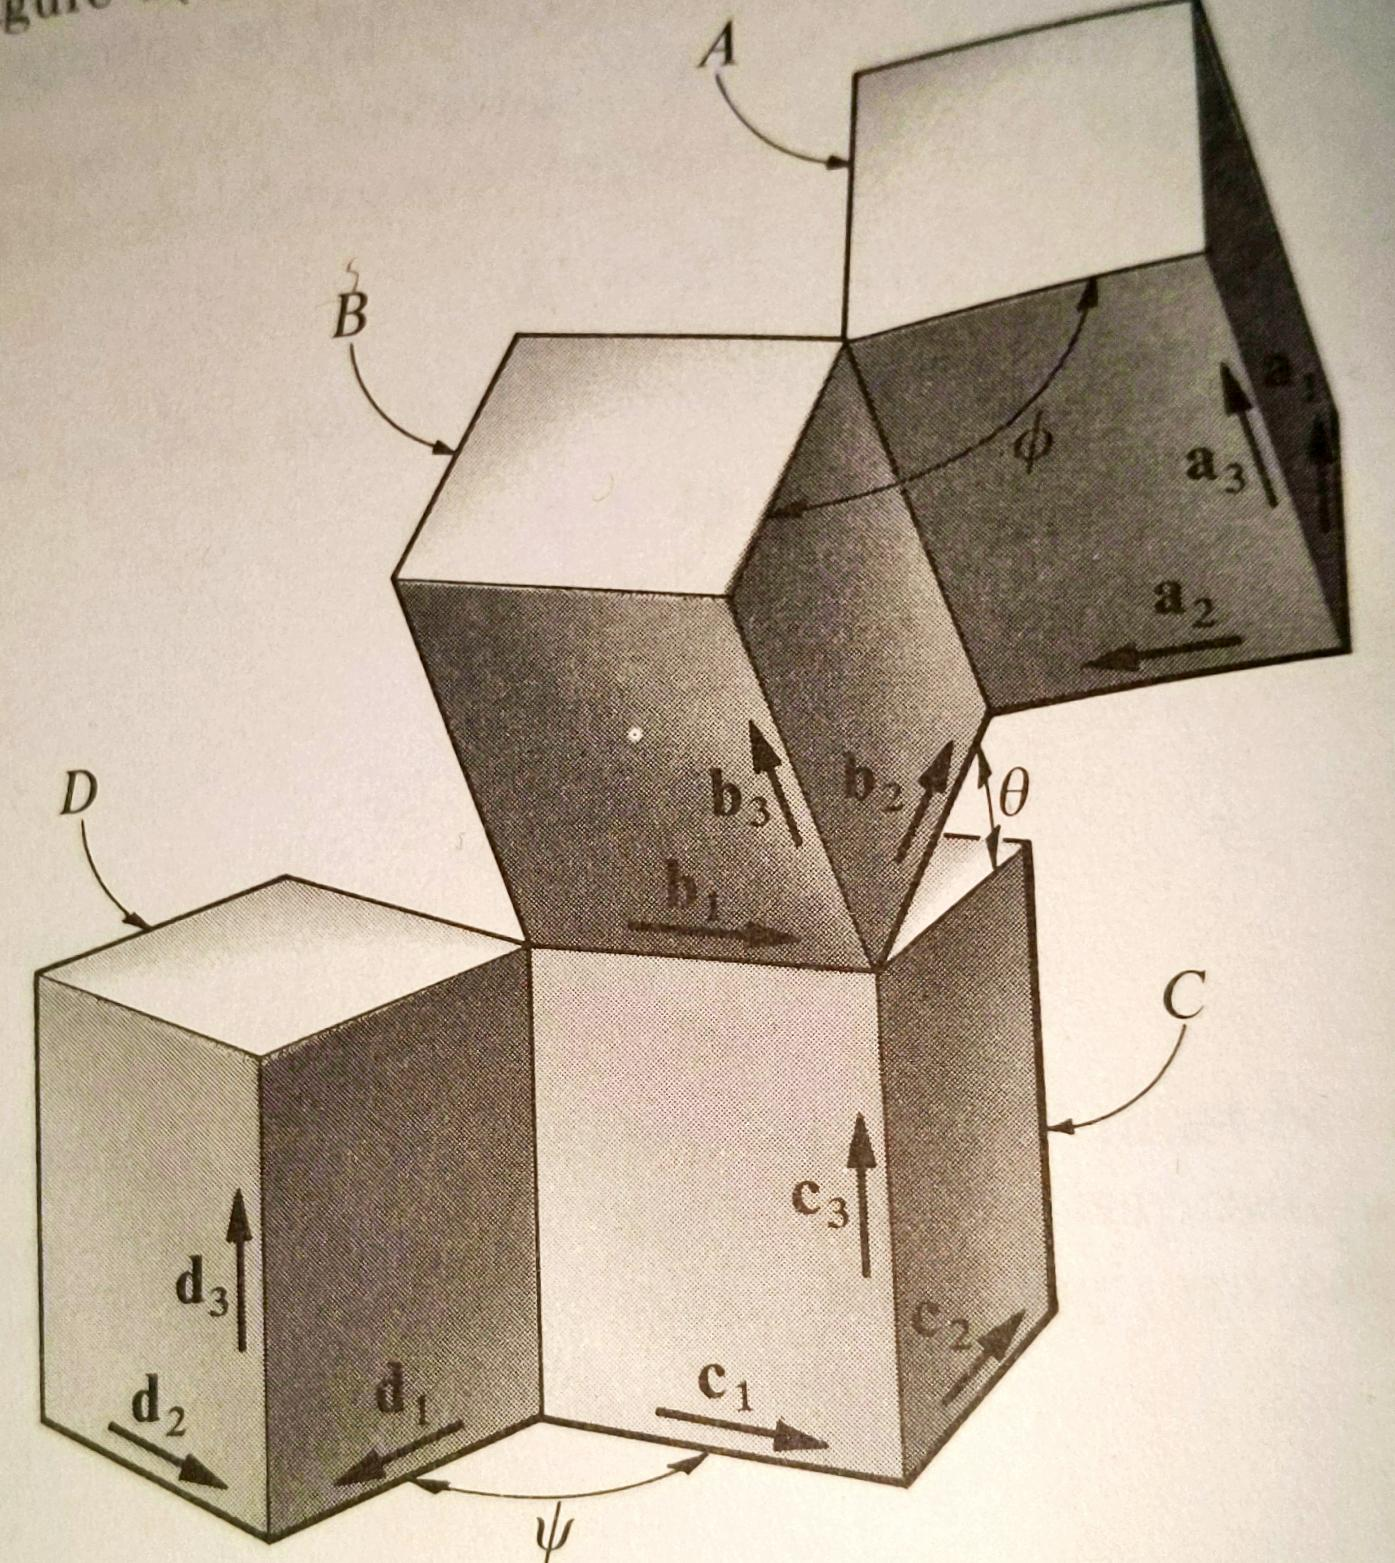
\includegraphics[width = 0.5\textwidth, height = 0.5\textwidth]{./figs/ProbSet_1/1_a.jpg}
    \caption{}
    \label{1_a}
\end{figure}


\textbf{\textit{sol.}}\\

We have the following rotation matrices:

\begin{align*}
     &\lx{^B}{\bm{\pmb a_1 \\ \pmb a_2 \\ \pmb a_3}} =
     \underbrace{
        \bm{
            \cos \phi & \sin \phi  & 0\\
            -\sin \phi & \cos \phi & 0\\
            0          & 0         & 1
        }
     } _ {R_3 (\phi)}
    \lx{^B}{\bm{\pmb b_1 \\ \pmb b_2 \\ \pmb b_3}} ;\:
    %===
    \lx{^C}{\bm{\pmb b_1 \\ \pmb b_2 \\ \pmb b_3}} =
    \underbrace{
        \bm{
            1 & 0 & 0\\
            0 & \cos \theta & \sin \theta\\
            0 & -\sin \theta & \cos \theta
        }
     } _ {R_1 (\theta)}
    \lx{^C}{\bm{\pmb c_1 \\ \pmb c_2 \\ \pmb c_3}} ;\:
    %===
    \lx{^D}{\bm{\pmb c_1 \\ \pmb c_2 \\ \pmb c_3}} =
     \underbrace{
        \bm{
            \cos \psi & \sin \psi  & 0\\
            -\sin \psi & \cos \psi & 0\\
            0          & 0         & 1
        }
     } _ {R_3 (\psi)}
    \lx{^D}{\bm{\pmb d_1 \\ \pmb d_2 \\ \pmb d_3}} \\
    %===
    &\text{Let, } \qquad
    \pmb a = \bm{\pmb a_1 \\ \pmb a_2 \\ \pmb a_3} \quad
    \pmb b = \bm{\pmb b_1 \\ \pmb b_2 \\ \pmb b_3} \quad
    \pmb c = \bm{\pmb c_1 \\ \pmb c_2 \\ \pmb c_3} \quad
    \pmb d = \bm{\pmb d_1 \\ \pmb d_2 \\ \pmb d_3}
\end{align*}

Thus, we have,

\begin{enumerate}
 \item
 \begin{align*}
   \lx{^B}{\frac {\partial \pmb a_1}  {\partial \phi}}&=
   %=
   \frac{\partial}{\partial \phi} \left(R_3(\phi)[1, :]  \times \lx{^B}{\pmb b} \right)
   %=
   = \frac{\partial R_3(\phi)[1, :]}{\partial \phi} \lx{^B}{\pmb b}
   %=
   \qquad \left[\because \pmb b_1, \pmb b_2,  \pmb b_3
   \text{ are fixed in } B \right]\\
   %=
   &= \bm{-\sin \phi & cos \phi & 0}
    \times \lx{^B}{\pmb b}\\
    %===
    &\implies \lx{^B}{\norm{\frac {\partial \pmb a_1}  {\partial \phi}}} = 1
 \end{align*}

 \item
 \begin{align*}
    \lx{^B}{\frac {\partial \pmb b_1}  {\partial \phi}} &= 0
    %=
    \implies \lx{^B}{\norm{ \frac {\partial \pmb b_1}  {\partial \phi}}} = 0
    %=
   \qquad \left[\because \pmb b_1, \pmb b_2,  \pmb b_3
   \text{ are fixed in } B \right]\\
 \end{align*}

 \item
 \begin{align*}
    \lx{^B}{\frac {\partial \pmb a_3}  {\partial \phi}} &=
   %=
   \frac{\partial}{\partial \phi} \left(R_3(\phi)[3, :]  \times \lx{^B}{\pmb b} \right)
   %=
   = \frac{\partial \pmb b_3}{\partial \phi}
   = 0
   %=
   \qquad \left[\because \pmb b_1, \pmb b_2,  \pmb b_3
   \text{ are fixed in } B \right]\\
   %===
   &\implies \lx{^B}{\norm{\frac {\partial \pmb a_3}  {\partial \phi}}} = 0
 \end{align*}


 \item
 \begin{align*}
    \lx{^B}{\frac {\partial \pmb b_2}  {\partial \theta}} &= 0
    \implies \lx{^B}{\norm{\frac {\partial \pmb b_2}  {\partial \theta}}} = 0
    \qquad \left[\because \pmb b_1, \pmb b_2,  \pmb b_3
   \text{ are fixed in } B \right]\\
 \end{align*}

\item
\begin{align*}
    \lx{^C}{\frac {\partial \pmb b_2}  {\partial \theta}} &= \frac {\partial}  {\partial \theta} \left( R_1(\theta)[2,:] \times \lx{^C}{\pmb c} \right)
    = \frac{\partial R_1(\theta)[2,:]}{\partial \theta} \times \lx{^C}{\pmb c}
    \qquad \left[\because \pmb c_1, \pmb c_2, \pmb c_3 \text{ are fixed in } C \right]\\
    %==
    &= \bm{0 & -\sin \theta & \cos \theta} \times \lx{^C}{\pmb c}\\
    %===
    &\implies \lx{^C}{\norm{\frac {\partial \pmb b_2}  {\partial \theta}}} = 1
\end{align*}


 \item
 \begin{align*}
    \lx{^D}{\frac {\partial \pmb b_2}  {\partial \theta}} &= \frac {\partial}  {\partial \theta} \left((R_1(\theta) R_3(\psi))[2,:] \times \lx{^D}{\pmb d} \right)
    \qquad \left[\because \pmb d_1, \pmb d_2, \pmb d_3 \text{ are fixed in } D \right]\\
    %===
    &= \frac{\partial (R_1(\theta) R_3(\psi))[2,:]}{\partial \theta} \lx{^D}{\bm{\pmb d_1 \\ \pmb d_2 \\ \pmb d_3}}
    %===
    = \left(\frac{\partial R_1(\theta) }{\partial \theta} R_3(\psi) \right) [2,:]\lx{^D}{\pmb d}
    %===
    = \left(\frac{\partial R_1(\theta)[2,:] }{\partial \theta} R_3(\psi) \right)\lx{^D}{\pmb d}\\
    %===
    &=  \left( \bm{0 & -\sin \theta & \cos \theta}
    \bm{
            \cos \psi & \sin \psi  & 0\\
            -\sin \psi & \cos \psi & 0\\
            0          & 0         & 1
        } \right)\lx{^D}{\pmb d}
    %===
    = \bm{\sin \theta \sin \psi & -\sin \theta \cos \psi & \cos \theta} \lx{^D}{\pmb d}\\
    %===
    &\implies  \lx{^D}{\norm{\frac {\partial \pmb b_2}  {\partial \theta}}} = 1
 \end{align*}

 \item
\begin{align*}
    \lx{^C}{\frac {\partial \pmb b_2}  {\partial \psi}} &= 0
    \implies \lx{^C}{\norm{\frac {\partial \pmb b_2}  {\partial \psi}}} = 0
    \qquad \left[ \because \text{Any vector defined in C is independent of } \psi \right]
\end{align*}

 \item
\begin{align*}
    \lx{^D}{\frac {\partial \pmb b_2}  {\partial \psi}} &= \frac{\partial}{\partial \psi} \left((R_1(\theta) R_3(\psi))[2,:] \times \lx{^D}{\pmb d} \right)
    \qquad \left[\because \pmb d_1, \pmb d_2, \pmb d_3 \text{ are fixed in } D \right]\\
    %==
    &= R_1(\theta)[2,:] \times \frac{\partial R_3(\psi)}{\partial \psi} \times \lx{^D}{\pmb d}
    %==
    = \bm{0 & \cos \theta & \sin \theta} \bm{-\sin \psi & \cos \psi & 0 \\
                                             -\cos \psi & -\sin \psi & 0\\
                                             0 & 0 & 0}
                        \times \lx{^D}{\pmb d}\\
    %==
    &= \bm{-\cos \theta \cos \psi & -\cos \theta \sin \psi & 0} \times \lx{^D}{\pmb d}\\
    %==
    &\implies  \lx{^D}{\norm{\frac {\partial \pmb b_2}  {\partial \psi}}} = \norm{\cos \theta}
\end{align*}

\item
\begin{align*}
    \lx{^D}{\frac {\partial \pmb a_1}  {\partial \psi}} &=  \frac{\partial}{\partial \psi} \left((R_3(\phi)R_1(\theta) R_3(\psi))[2,:] \times \lx{^D}{\pmb d} \right)
    %==
    = R_3(\phi)[1,:] \times R_1(\theta) \times \frac{\partial R_3(\psi)}{\partial \psi} \times \lx{^D}{\pmb d}\\
    %==
    %\quad \left[\because \pmb d_1, \pmb d_2, \pmb d_3 \text{ are fixed in } D \right]\\
    %==
    &= \bm{\cos \phi & \sin \phi  & 0}
      \bm{
            1 & 0 & 0\\
            0 & \cos \theta & \sin \theta\\
            0 & -\sin \theta & \cos \theta
        }
      \bm{
            -\sin \psi & \cos \psi  & 0\\
            -\cos \psi & -\sin \psi & 0\\
            0          & 0         & 0
        }\lx{^D}{\pmb d}\\
    %==
    &= \bm{-\cos \phi \sin \psi - \sin \phi \cos \theta \cos \psi &
          \cos \phi \cos \psi - \sin \phi \cos \theta \sin \psi &
          0} \lx{^D}{\pmb d}\\
    %==
     \implies \lx{^D}{\norm{\frac {\partial \pmb a_1}  {\partial \psi}}} &=
    \sqrt{(-\cos \phi \sin \psi - \sin \phi \cos \theta \cos \psi )^2 +
    (\cos \phi \cos \psi - \sin \phi \cos \theta \sin \psi )^2}\\
    %==
    &= (\cos^2 \phi + \sin^2\phi \sin^2 \theta)^{1/2}
\end{align*}

\end{enumerate}

\subsection{1(b)}
\textbf{\textit{Problem}}: Referring to Problem $1(a)$, determine $w_1, w_2$ and  $w_3$ such that
$$ \lx{^C}{\frac{\partial \pmb a_1}{\partial \theta}} = w_1 \pmb a_1 + w_2 \pmb a_2 + w_3 \pmb a_3$$

\textbf{\textit{sol.}}

We have,
\begin{align*}
    \lx{^C}{\frac{\partial \pmb a_1}{\partial \theta}}  &=
    \frac{\partial}{\partial \theta} [R_3(\phi)[1,:]R_1(\theta)] \times \lx{^C}{\pmb c}
    %==
    = R_3(\phi)[1,:] \frac{\partial R_1(\theta)}{\partial \theta} \times \lx{^C}{\pmb c}
    %===
    = R_3(\phi)[1,:] \frac{\partial R_1(\theta)}{\partial \theta} \times [R_3(\phi)R_1(\theta)]^{-1} \times \lx{^C}{\pmb a}\\
    %==
    &=R_3(\phi)[1,:] \frac{\partial R_1(\theta)}{\partial \theta} \times R_1^T(\theta) R_3^T(\phi)\times \lx{^C}{\pmb a}
    %==
    \qquad \left[ \because R_i^{-1} = R_i^T \right]\\
    %==
    &= \bm{\cos \phi & \sin \phi  & 0}
    \bm{
            0 & 0 & 0\\
            0 & -\sin \theta & \cos \theta\\
            0 & -\cos \theta & -\sin \theta
        }
    \bm{
            1 & 0 & 0\\
            0 & \cos \theta & -\sin \theta\\
            0 & \sin \theta & \cos \theta
    }
    \bm{
            \cos \phi & -\sin \phi  & 0\\
            \sin \phi & \cos \phi & 0\\
            0          & 0         & 1
        }
    \times \lx{^c}{\pmb a}\\
     %==
    &= \bm{\cos \phi & \sin \phi  & 0}
    \bm{
            0 & 0 & 0\\
            0 & 0 & 1\\
            0 & 1 & 0
        }
    \bm{
            \cos \phi & -\sin \phi  & 0\\
            \sin \phi & \cos \phi & 0\\
            0          & 0         & 1
        }
    \times \lx{^c}{\pmb a}
    %==
    = \bm{0 & 0 & \sin \phi} \times \lx{^c}{\pmb a}\\
    %==
    \text{Hence, }&\\
    & w_1 = w_2 = 0, \: w_3 = \sin \phi
\end{align*}

\subsection{1(c)}
\textbf{\textit{Problem}}: Referring to Problem~$1(a)$, and assuming that $\theta, \phi$ and $\psi$ are functions of the time $t$ such that, at a certain instant $t^*$, $\phi = \theta = \psi = \pi/6 \; rad$, $\dot \phi = 4 \; rad/sec$, and $\dot \theta = \dot \psi = 6 \; rad/sec$, show that at time $t^*$,
$$ \lx{^C}{\frac{\partial \pmb a_1}{\partial t}} = 4 \pmb a_2 + 3 \pmb a_3$$

\textbf{\textit{sol.}}

We have,
\begin{align*}
    \lx{^C}{{\pmb a_1}} &= R_3(\phi)[1, :] R_1(\theta) \times \lx{^C}{\pmb c}\\
    \\
    %===
    \implies \lx{^C}{\frac{d \pmb a_1}{dt}} &= \left( \frac{\partial R_3(\phi)[1, :]}{\partial \phi}   R_1(\theta) \dot \phi + R_3(\phi)[1, :] \frac{\partial R_1(\theta)}{\partial \theta } \dot \theta \right) \times \lx{^C}{\pmb c}\\
    %===
    &= \left( \frac{\partial R_3(\phi)[1, :]}{\partial \phi}   R_1(\theta) \dot \phi + R_3(\phi)[1, :] \frac{\partial R_1(\theta)}{\partial \theta } \dot \theta \right) \times R_1^T(\theta) R_3^T(\phi) \times \lx{^C}{\pmb a}\\
    %==
    &= \left[
    \left(\frac{\partial R_3(\phi)[1, :]}{\partial \phi}   R_3^T(\phi)
    \right)\dot \phi +
    \left(R_3(\phi)[1, :] \frac{\partial R_1(\theta)}{\partial \theta } R_1^T(\theta) R_3^T(\phi)
    \right) \dot \theta
    \right]\times \lx{^C}{\pmb a}\\
    %==
    &= \left[
    \left(\bm{-\sin \phi & \cos \phi & 0}\bm{
            \cos \phi & -\sin \phi  & 0\\
            \sin \phi & \cos \phi & 0\\
            0          & 0         & 1
        }
    \right)\dot \phi +
    \left(\bm{0 & 0 & \sin \phi}
    \right) \dot \theta
    \right]\times \lx{^C}{\pmb a}
    %==
    \qquad \left[\text{From } 1(b) \right]\\
    %==
    &= \left( \bm{0&1&0} \dot \phi + \bm{0 & 0 & \sin \phi} \dot \theta \right) \lx{^C}{{\pmb a}}\\
    %===
    \\
    \text{Substituting }&\; \phi = \frac{\pi}{6} \: \dot \phi =4 \; \dot \theta = 6\\
    %===
    \implies \lx{^C}{\frac{d \pmb a_1}{dt}} &= 4 \pmb a_2 + 3 \pmb a_3
\end{align*}

\subsubsection{1(d)}
\textbf{\textit{Problem}}: In Figure~\ref{1_d}, N designates a plane that is made to rotate with constant angular speed $\omega$ about a line $Z$ fixed in $N$ and in a reference frame $R$. The unit vectors $\pmb n_x, \pmb n_y$ and  $\pmb n_z$ are mutually perpendicular and fixed in R, and $\pmb n$ is a unit vector normal to $N$ and equal to $\pmb n_x$ at time $t=0$. Finally, $P_1$ and $P_2$ represent particles connected to each other by a rigid rod of lenghth $L$, these particles remaining at all times in contact with $N$.

\begin{figure}[H]
    \centering
    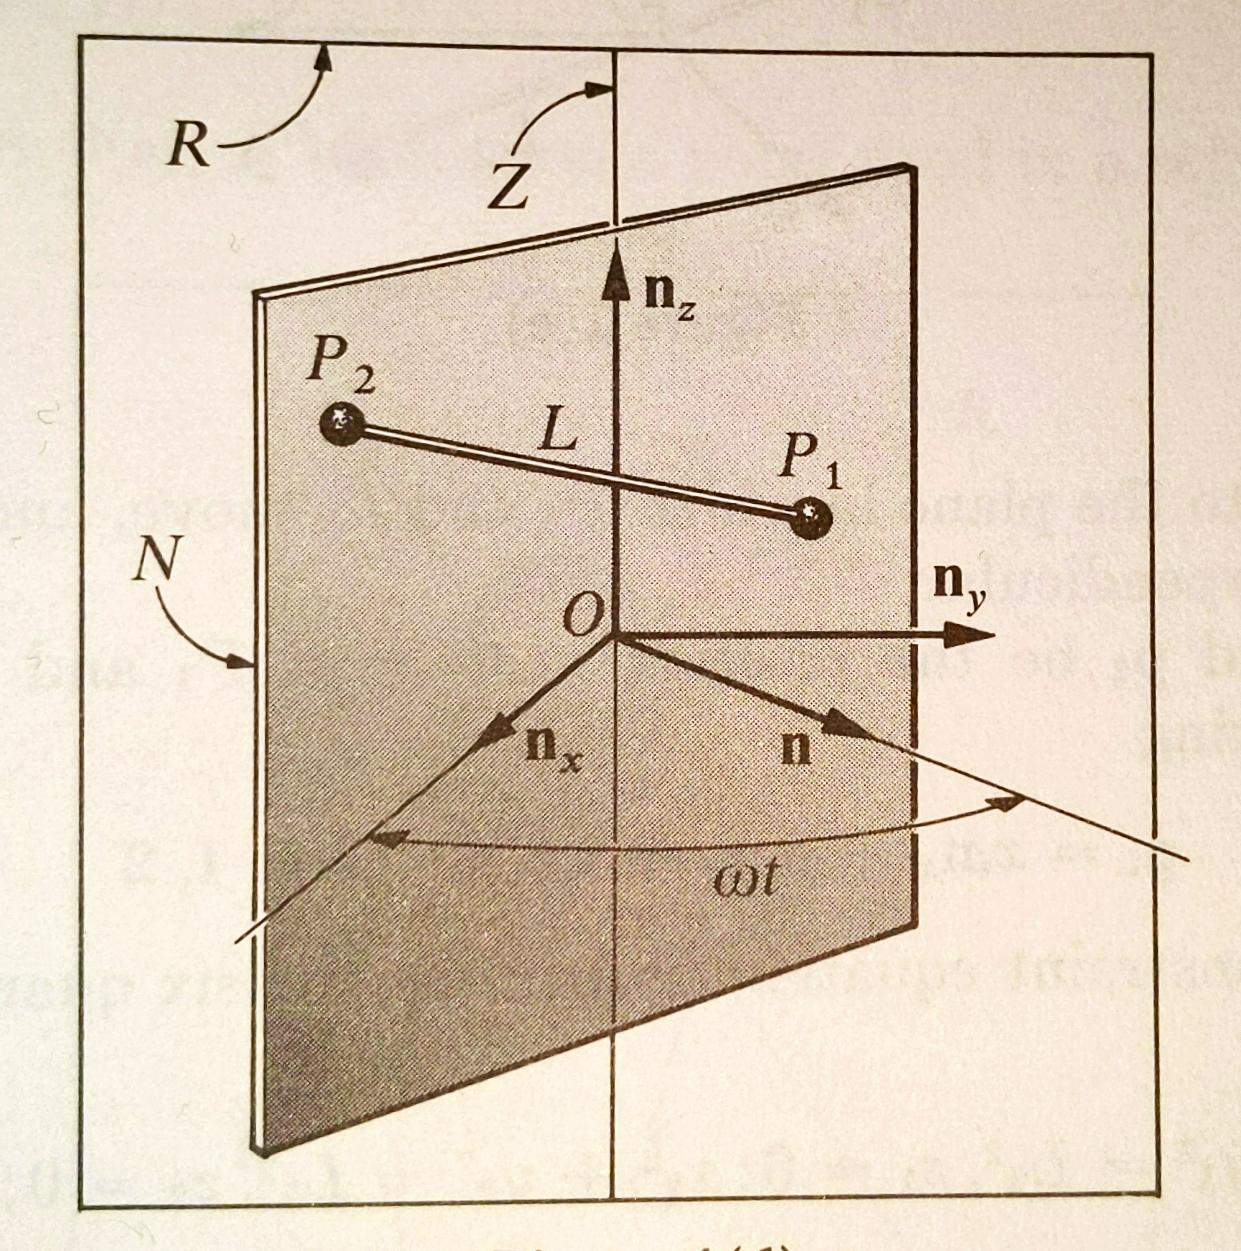
\includegraphics[width = 0.35\textwidth, height = 0.3\textwidth]{figs/ProbSet_1/1_d.jpg}
    \caption{}
    \label{1_d}
\end{figure}


Letting $\pmb p_1$ and $\pmb p_2$ be the position vectors of $P_1$ and $P_2$ relative to a point $O$ fixed in line $Z$, and taking

$$\pmb p_i = x_i \pmb n_x + y_i \pmb n_y + z_i \pmb n_z \qquad i = 1, 2$$

detarmine functions $f_j(x_1, y_1, z_1, x_2, y_2, z_2, t)$, for $j=1, 2, 3$, such that the requirements that $P_1$ and $P_2$ remain in $N$ and be separated by distance $L$ can be experessed as $f_j = 0$, $j = 1, 2, 3$.

\textbf{\textit{Sol.}}:

\begin{enumerate}
    \item For $P_1$ and $P_2$ to be attached to $N$ at all times,
    \begin{align*}
        \pmb p_i .  \pmb n &= 0 \quad \forall \; t, \qquad i = 1, 2\\
        \text{We have, } \qquad &\\
        \pmb n(t) &= \pmb n_x \sin \omega t + \pmb n_y \cos \omega t\\
        \\
        \implies \pmb p_i .  \pmb n &= x_i \sin \omega t + y_i \cos \omega t = 0 \qquad i=1, 2\\
        \\
        \therefore f_1 &= x_1 \sin \omega t + y_1 \cos \omega t\\
                   f_2 &= x_2 \sin \omega t + y_2 \cos \omega t
    \end{align*}

    \item For the distance between $P_1$ and $P_2$ to remain $L$:
    \begin{align*}
        \norm{\pmb p_1 - \pmb p_2} &= L\\
        \\
        \implies f_3 &= (x_1 - x_2)^2 + (y_1 - y_2)^2 + (z_1 - z_2)^2 - L^2
    \end{align*}
\end{enumerate}

\subsection{1(e)}

\subsection{1(f)}
\itbf{Problem}: Referring to Problem~$1(d)$, and letting S be the set of particles $P_1$ and $P_2$, determine the number of degrees of freedom of $S$ in $R$.

\itbf{Sol.}:

We have 3 constraint eqautions $(M=3)$ and 2 particles $(N=2)$. The number of degrees of freedom:
$$3N-M = 3 \times 2 - 3 = 3$$

\subsection{1(g) Generalized coordinates.}
\itbf{Problem}: Referring to the Problem~$1(e)$, express the six quantities
$x_i, y_i, z_i$ with $i=1,2$, each as a function of a single quantity $q$ in
such a way that the five constraint equations found previously are satisfied for
all values of $q$. (Suspension: Let $q$ be the radian measure of the angle
between $\pmb n_x$ and $\pmb p_2$.)

\itbf{Sol.}:

\begin{multicols}{2}
\begin{align*}
    x_1 &= -L_1 \cos q\\
    y_1 &= L_1 \sin q\\
    z_1 &=  0
\end{align*}

\begin{align*}
    x_2 &= L_2 \cos q\\
    y_2 &= -L_2 \sin q\\
    z_2 &=  0
\end{align*}
\end{multicols}

\subsection{1(h)}

\itbf{Problem}: Determine the number of degrees of freedom of each of the following holonomic systems:

\itbf{Sol.}:

\begin{enumerate}
    \item Two rigid bodies attached to each other by means of a ball-and-socket connedtion.

    --The position of both the bodies is constrained but not the orientations of the individaul bodies.
    $$n=9$$

    \item An earth satellite carrying a rotor that is made to ratate at a prescribed rate about an axis fixed in the satellite.

    -- All dof's of the rotor are constrained to that of satellite except the rotation about it's axis which is also constrained as it's rate is prescribed.
    $$n = 6$$

    \item An earth satellite carrying a rotor that is made to ratate at a prescribed rate about an axis fixed in the satellite.

    -- All dof's of the rotor are constrained to that of satellite except the rotation about it's axis.
    $$n = 7$$

    \item The particles $P_1, P_2$ of Problem~$1(e)$.

    -- The only degree of freedom is the rotation about $\pmb n_z$.
    $$n=1$$
\end{enumerate}

%===============================================================================
\newpage
\section{Problem Set 2}
\subsection{2(a)}

\itbf{Problem}: In Figure~\ref{2_a}, P represents a point fixed in a reference frame R, and $B^*$ designates the mass center of a rigid body $B$ that moves on a circular orbit $C$ fixed in $R$ and centered at $P$. $A_1, A_2$ and $A_3$ are mutually perpendicular directed line segments, $A_1$ being the extension of line $PB^*$, $A_2$ pointing in the direction of motion of $B^*$ on $C$, and $A_3$ thus being normal to the plane of the orbit $B^*$.

\begin{figure}[H]
    \centering
    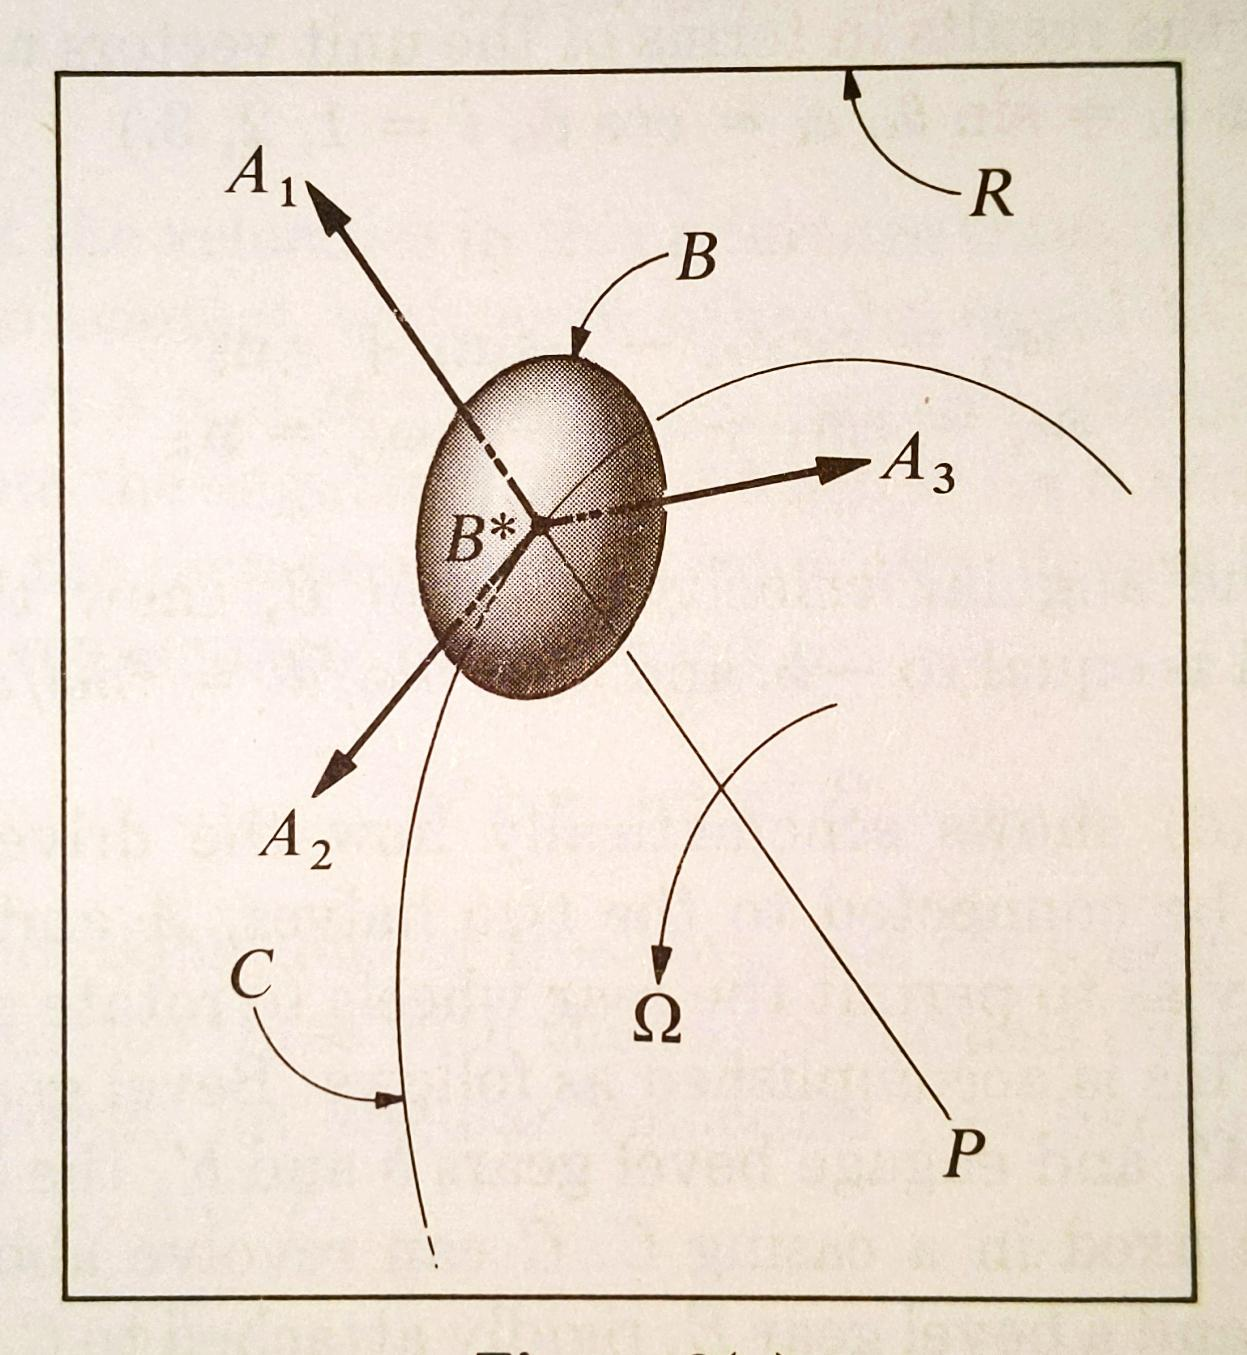
\includegraphics[scale = 0.15]{./figs/ProbSet_2/2_a.jpg}
    \caption{}
    \label{2_a}
\end{figure}

If $X_1, X_2$ and $X_3$ are mutually perpendicular directed line segments passing through $B^*$ and fixed in the body $B$, the "attitude" of $B$ relative to $A_1, A_2, A_3$ can be specified in terms of three angles $\theta_1, \theta_2$ and $\theta_3$, generated as follows: \itbf{Align $X_i$ with $A_i$, for $i=1, 2, 3$, and perform successive right-handed rotations of $B$, of amount $\theta_1$ about $X_1$, $\theta_2$ about $X_2$, and $\theta_3$ about $X_3$.}

The angular velocity $\pmb \omega$ of $B$ in $R$ can be expressed as $\pmb \omega = \omega_1 \pmb n_1 + \omega_2 \pmb n_2 + \omega_3 \pmb n_3$, where $\pmb n_i$ is a unit vector parallel to $X_i$, and $\omega_i$ is a function of $\theta_1, \theta_2, \theta_3, \dot \theta_1, \dot \theta_2, \dot \theta_3$, and the anglular speed $\Omega$ of the line $PB^*$ in R. Consequently, $\dot \theta_i$ can be expressed as a function $f_i$ of $\theta_1, \theta_2, \theta_3, \omega_1, \omega_2, \omega_3$, $i = 1,2,3$ and $\Omega$.

Determine the functions $f_1, f_2$ and $f_3$, using the abbrivations $s_i = \sin \theta_i, c_i = \cos \theta_i$ for $i = 1,2,3$, to state the results.\\

\itbf{Sol.}:\\

\itbf{Note}: The above explanation of $X_1, X_2$ and $X_3$ is the loose definition of Euler angles used to define the orientation of a rigid body.\\

\itbf{Rotation Matrices}:

The given description of obtaining the attitude of the body can be put mathematically uising rotation matrices as follows:

\begin{multicols}{2}
 \begin{enumerate}
    \item Right-handed rotation about $X_1$ by $\theta_1$:
    \begin{align*}
        \bm{X_1\\ X_2\\ X_3^{'}} &=
        \underbrace{\bm{1 & 0 & 0\\
                        0 & c_1 & s_1\\
                        0 & -s_1 & c_1}}_{R_1}
        \bm{A_1\\ A_2\\ A_3}
    \end{align*}
    \item Right-handed rotation about $X_2$ by $\theta_2$:
    \begin{align*}
        \bm{X_1^{'}\\ X_2\\ X_3} &=
        \underbrace{\bm{c_2 & 0 & -s_2\\
                        0 & 1 & 0\\
                        s_2 & 0 & c_2}}_{R_2}
        \bm{X_1\\ X_2\\ X_3^{'}}
    \end{align*}
    \item Right-handed rotation about $X_3$ by $\theta_3$:
    \begin{align*}
        \bm{X_1^{''}\\ X_2^{'}\\ X_3} &=
        \underbrace{\bm{c_3 & s_3 & 0\\
                        -s_3 & c_3 & 0\\
                        0 & 0 & 1}}_{R_3}
        \bm{X_1^{'}\\ X_2\\ X_3}
    \end{align*}
\end{enumerate}

\itbf{Interpretation}: $\pmb n_i$ are the unit vectors parallel to $X_i$ after the above transformation sequence.\\
Thus,
\begin{align*}
    \bm{\pmb n_1 \\ \pmb n_2 \\ \pmb n_3} &= \bm{X_1^{''}\\ X_2^{'}\\ X_3}
\end{align*}
\end{multicols}

We have, the (instantaneous) angular velocity of the body in $A$ frame:
\begin{align*}
    \lx{^A}{\pmb \omega}^B &= \dot \theta_1 X_1 + \dot \theta_2 X_2 + \dot \theta_3 X_3
\end{align*}

The angular velocity of $A$ in $R$:
$$ \lx{^R}{\pmb \omega}^A = \Omega A_3$$

The angular velocity of the body in reference frame:
\begin{align*}
    \lx{^R}{\pmb \omega}^B &= \lx{^R}{\pmb \omega}^A + \lx{^A}{\pmb \omega}^B\\
        &= \Omega A_3 +\dot \theta_1 X_1 + \dot \theta_2 X_2 + \dot \theta_3 X_3
\end{align*}

Requried form:
\begin{align*}
    \lx{^R}{\pmb \omega}^B &= \omega_1 \pmb n_1 + \omega_2 \pmb n_2 + \omega_3 \pmb n_3
\end{align*}

Thus we need to write $A_3, X_1, X_2$ and $X_3$ in terms of $\pmb n_1, \pmb n_2, \pmb n_3$.

\begin{multicols}{2}
From the third transformation:
\begin{align*}
    \bm{X_1^{'}\\ X_2\\ X_3} &=
                    \bm{c_3 & -s_3 & 0\\
                        s_3 & c_3 & 0\\
                        0 & 0 & 1}
    \bm{\pmb n_1 \\ \pmb n_2 \\ \pmb n_3}\\
    \implies X_2 &= s_3 \pmb n_1 + c_3 \pmb n_2 \qquad X_3 = \pmb n_3\\
         X_1^{'} &= c_3 \pmb n_1 - s_3 \pmb n_2
\end{align*}
From the second transformation:
\begin{align*}
    \bm{X_1\\ X_2\\ X_3^{'}} &=
        \bm{c_2 & 0 & s_2\\
            0 & 1 & 0\\
            -s_2 & 0 & c_2}
    \bm{X_1^{'}\\ X_2\\ X_3}\\
    \implies X_1 &= c_2 X_1^{'} + s_2 X_3\\
    \implies X_1 &= c_2(c_3 \pmb n_1 - s_3 \pmb n_2) + s_2 \pmb n_3
\end{align*}
\end{multicols}

\begin{align*}
    \bm{X_1\\ X_2\\ X_3} &= \underbrace{\bm{c_2 c_3 & -c_2 s_3 & s_2\\
                                s_3     & c_3      & 0\\
                                0       & 0        & 1}}_T
                            \bm{\pmb n_1 \\ \pmb n_2 \\ \pmb n_3}
\end{align*}

From the first transformation:
\begin{align*}
    \bm{A_1\\ A_2\\ A_3} &=
                    \bm{1 & 0 & 0\\
                        0 & c_1 & -s_1\\
                        0 & s_1 & c_1}
    \bm{X_1\\ X_2\\ X_3^{'}}
    \quad and \quad X_3^{'} = -s_2 X_1^{'} + c_2 X_3 = -s_2 (c_3 \pmb n_1 - s_3 \pmb n_2) + c_2 \pmb n_3\\
    \\
    \implies A_3 &= s_1 X_2 + c_1 X_3^{'} = s_1(s_3 \pmb n_1 + c_3 \pmb n_2 ) + c_1 (-s_2 (c_3 \pmb n_1 - s_3 \pmb n_2) + c_2 \pmb n_3)\\
    &= \underbrace{\bm{s_1 s_3 - c_1s_2c_3 & s_1c_3 + c_1 s_2 s_3 & c_1 c_2}}_{P^T}
        \bm{\pmb n_1 \\ \pmb n_2 \\ \pmb n_3}
\end{align*}

Substituting, and writing in matrix form:
\begin{align*}
    \omega_1 \pmb n_1 + \omega_2 \pmb n_2 + \omega_3 \pmb n_3 &= \Omega A_3 +\dot \theta_1 X_1 + \dot \theta_2 X_2 + \dot \theta_3 X_3\\
    \bm{\omega_1 & \omega_2 & \omega_3}  \bm{\pmb n_1 \\ \pmb n_2 \\ \pmb n_3}
    &= \Omega P^T  \bm{\pmb n_1 \\ \pmb n_2 \\ \pmb n_3}
        + \bm{\dot \theta_1 & \dot \theta_2 & \dot \theta_3} T \bm{\pmb n_1 \\ \pmb n_2 \\ \pmb n_3}\\
    %===
    \implies \bm{\omega_1 \\ \omega_2 \\ \omega_3} &= \Omega P + T^T  \bm{\dot \theta_1 \\ \dot \theta_2 \\ \dot \theta_3}\\
    %===
    \implies \bm{\dot \theta_1 \\ \dot \theta_2 \\ \dot \theta_3} &= [T^T]^{-1} \left(\bm{\omega_1 \\ \omega_2 \\ \omega_3} - \Omega P \right)
\end{align*}
Symbolically solving (using sympy), we get:
\begin{align*}
    \bm{\dot \theta_1 \\ \dot \theta_2 \\ \dot \theta_3}&=
    \left[\begin{matrix}\frac{\Omega \sin{\left(\theta_{2} \right)} \cos{\left(\theta_{1} \right)} + \omega_{1} \cos{\left(\theta_{3} \right)} - \omega_{2} \sin{\left(\theta_{3} \right)}}{\cos{\left(\theta_{2} \right)}}\\- \Omega \sin{\left(\theta_{1} \right)} + \omega_{1} \sin{\left(\theta_{3} \right)} + \omega_{2} \cos{\left(\theta_{3} \right)}\\- \frac{\Omega \cos{\left(\theta_{1} \right)}}{\cos{\left(\theta_{2} \right)}} - \omega_{1} \cos{\left(\theta_{3} \right)} \tan{\left(\theta_{2} \right)} + \omega_{2} \sin{\left(\theta_{3} \right)} \tan{\left(\theta_{2} \right)} + \omega_{3}\end{matrix}\right]
\end{align*}

Thus,
\begin{align*}
    \bm{\dot \theta_1 \\ \dot \theta_2 \\ \dot \theta_3}&=
    \bm{(\omega_1 c_3 - \omega_2 s_3 + \Omega s_2 c_1)/c_2 \\
        \omega_1 s_3 + \omega_2 c_3 - \Omega s_1 \\
        [(\omega_2 s_3 - \omega_1 c_3)s_2 + \omega_3 c_2 - \Omega c_1]/c_2}
\end{align*}

Sympy Code:
\lstinputlisting[language=python, caption ={}]{./ProblemSets/ProbSet_2/2a.py}

\subsection{2(b) $\pmb \omega = \sum \pmb \omega_{\dot q_i} \dot q_i +  \pmb \omega_t$}

\itbf{Sol.}\\

Given,

The motion of $B^*$ on $C$ is prescribed (predeterimined) $\implies \Omega(t)$ is give.

We have angular velocity written interms of partial rates:
\begin{align*}
    \pmb \omega = \sum \pmb \omega_{\dot q_i} \dot q_i +  \pmb \omega_t
\end{align*}

We have from $2(a)$,
\begin{align*}
    \lx{^R}{\pmb \omega}^B &=
    \Omega(t) P^T  \bm{\pmb n_1 \\ \pmb n_2 \\ \pmb n_3}
        + \bm{\dot \theta_1 & \dot \theta_2 & \dot \theta_3} T \bm{\pmb n_1 \\ \pmb n_2 \\ \pmb n_3}\\
    %===
    P &= \bm{s_1 s_3 - c_1s_2c_3 \\ s_1c_3 + c_1 s_2 s_3 \\ c_1 c_2} \qquad
    T = \bm{c_2 c_3 & -c_2 s_3 & s_2\\
             s_3     & c_3      & 0\\
             0       & 0        & 1}
    %===
\end{align*}

Let, $\pmb n = \bm{\pmb n_1 & \pmb n_2 & \pmb n_3}^T$

Thus, we have the partial rates:
\begin{align*}
    \lx{^R}{\pmb \omega}^B_t &= \lx{^R}{\frac{\partial \pmb \omega^B}{\partial t}} = \dot \Omega P^T \pmb n\\
    %===
    \lx{^R}{\pmb \omega}^B_{\dot \theta_1} &= \lx{^R}{\frac{\partial \pmb \omega^B}{\partial \dot \theta_1}} = T[1,:] \pmb n = \bm{c_2 c_3 & -c_2 s_3 & s_2} \pmb n\\
    %===
    \lx{^R}{\pmb \omega}^B_{\dot \theta_2} &= \lx{^R}{\frac{\partial \pmb \omega^B}{\partial \dot \theta_2}} = T[2,:] \pmb n = \bm{s_3     & c_3      & 0} \pmb n\\
    %===
    \lx{^R}{\pmb \omega}^B_{\dot \theta_3} &= \lx{^R}{\frac{\partial \pmb \omega^B}{\partial \dot \theta_3}} = T[3,:] \pmb n = \bm{0&0&1} \pmb n\\
\end{align*}

\subsection{2(c) Prove that $\lx{^B}{\pmb \omega}^A = -\lx{^A}{\pmb \omega}^B$
but,
$\lx{^A}{d \pmb \omega \backslash d t}= \lx{^B}{{d \pmb \omega} \backslash {dt}}$
}

Given, $\lx{^B}{\pmb \omega}^A = \pmb \omega$.

Let, $\pmb v$ be a vector, then
\begin{align*}
    \lx{^B}{\frac{d \pmb v}{d t}} &= \lx{^A}{\frac{d \pmb v}{d t}} + \pmb \omega \times \pmb v
    %===
    \implies \lx{^A}{\frac{d \pmb v}{d t}}  = \lx{^B}{\frac{d \pmb v}{d t}} - \pmb \omega \times \pmb v\\
    %==-
    \text{but, }\quad \lx{^A}{\frac{d \pmb v}{d t}}  &= \lx{^B}{\frac{d \pmb v}{d t}} + \lx{^A}{\pmb \omega}^B \times v\\
    %==-
    \text{By comparision, }\quad  \lx{^A}{\pmb \omega}^B &= - \pmb \omega\\
     %==
    \therefore  \lx{^B}{\pmb \omega}^A &= \pmb \omega \implies \lx{^A}{\pmb \omega}^B = - \pmb \omega & q.e.d
\end{align*}

Using the operator definition of angular velocity vector on itself:
\begin{align*}
    \lx{^B}{\frac{d \pmb \omega }{d t}}  &= \lx{^A}{\frac{d \pmb \omega }{d t}} + \underbrace{\pmb \omega \times  \pmb \omega}_{=0} \\
    %==
    \therefore \lx{^B}{\frac{d \pmb \omega }{d t}}  &= \lx{^A}{\frac{d \pmb \omega }{d t}} &q.e.d\\
\end{align*}

\subsection{2(d) Differential gear and drive shaft kinematics}
\begin{figure}[H]
    \centering
    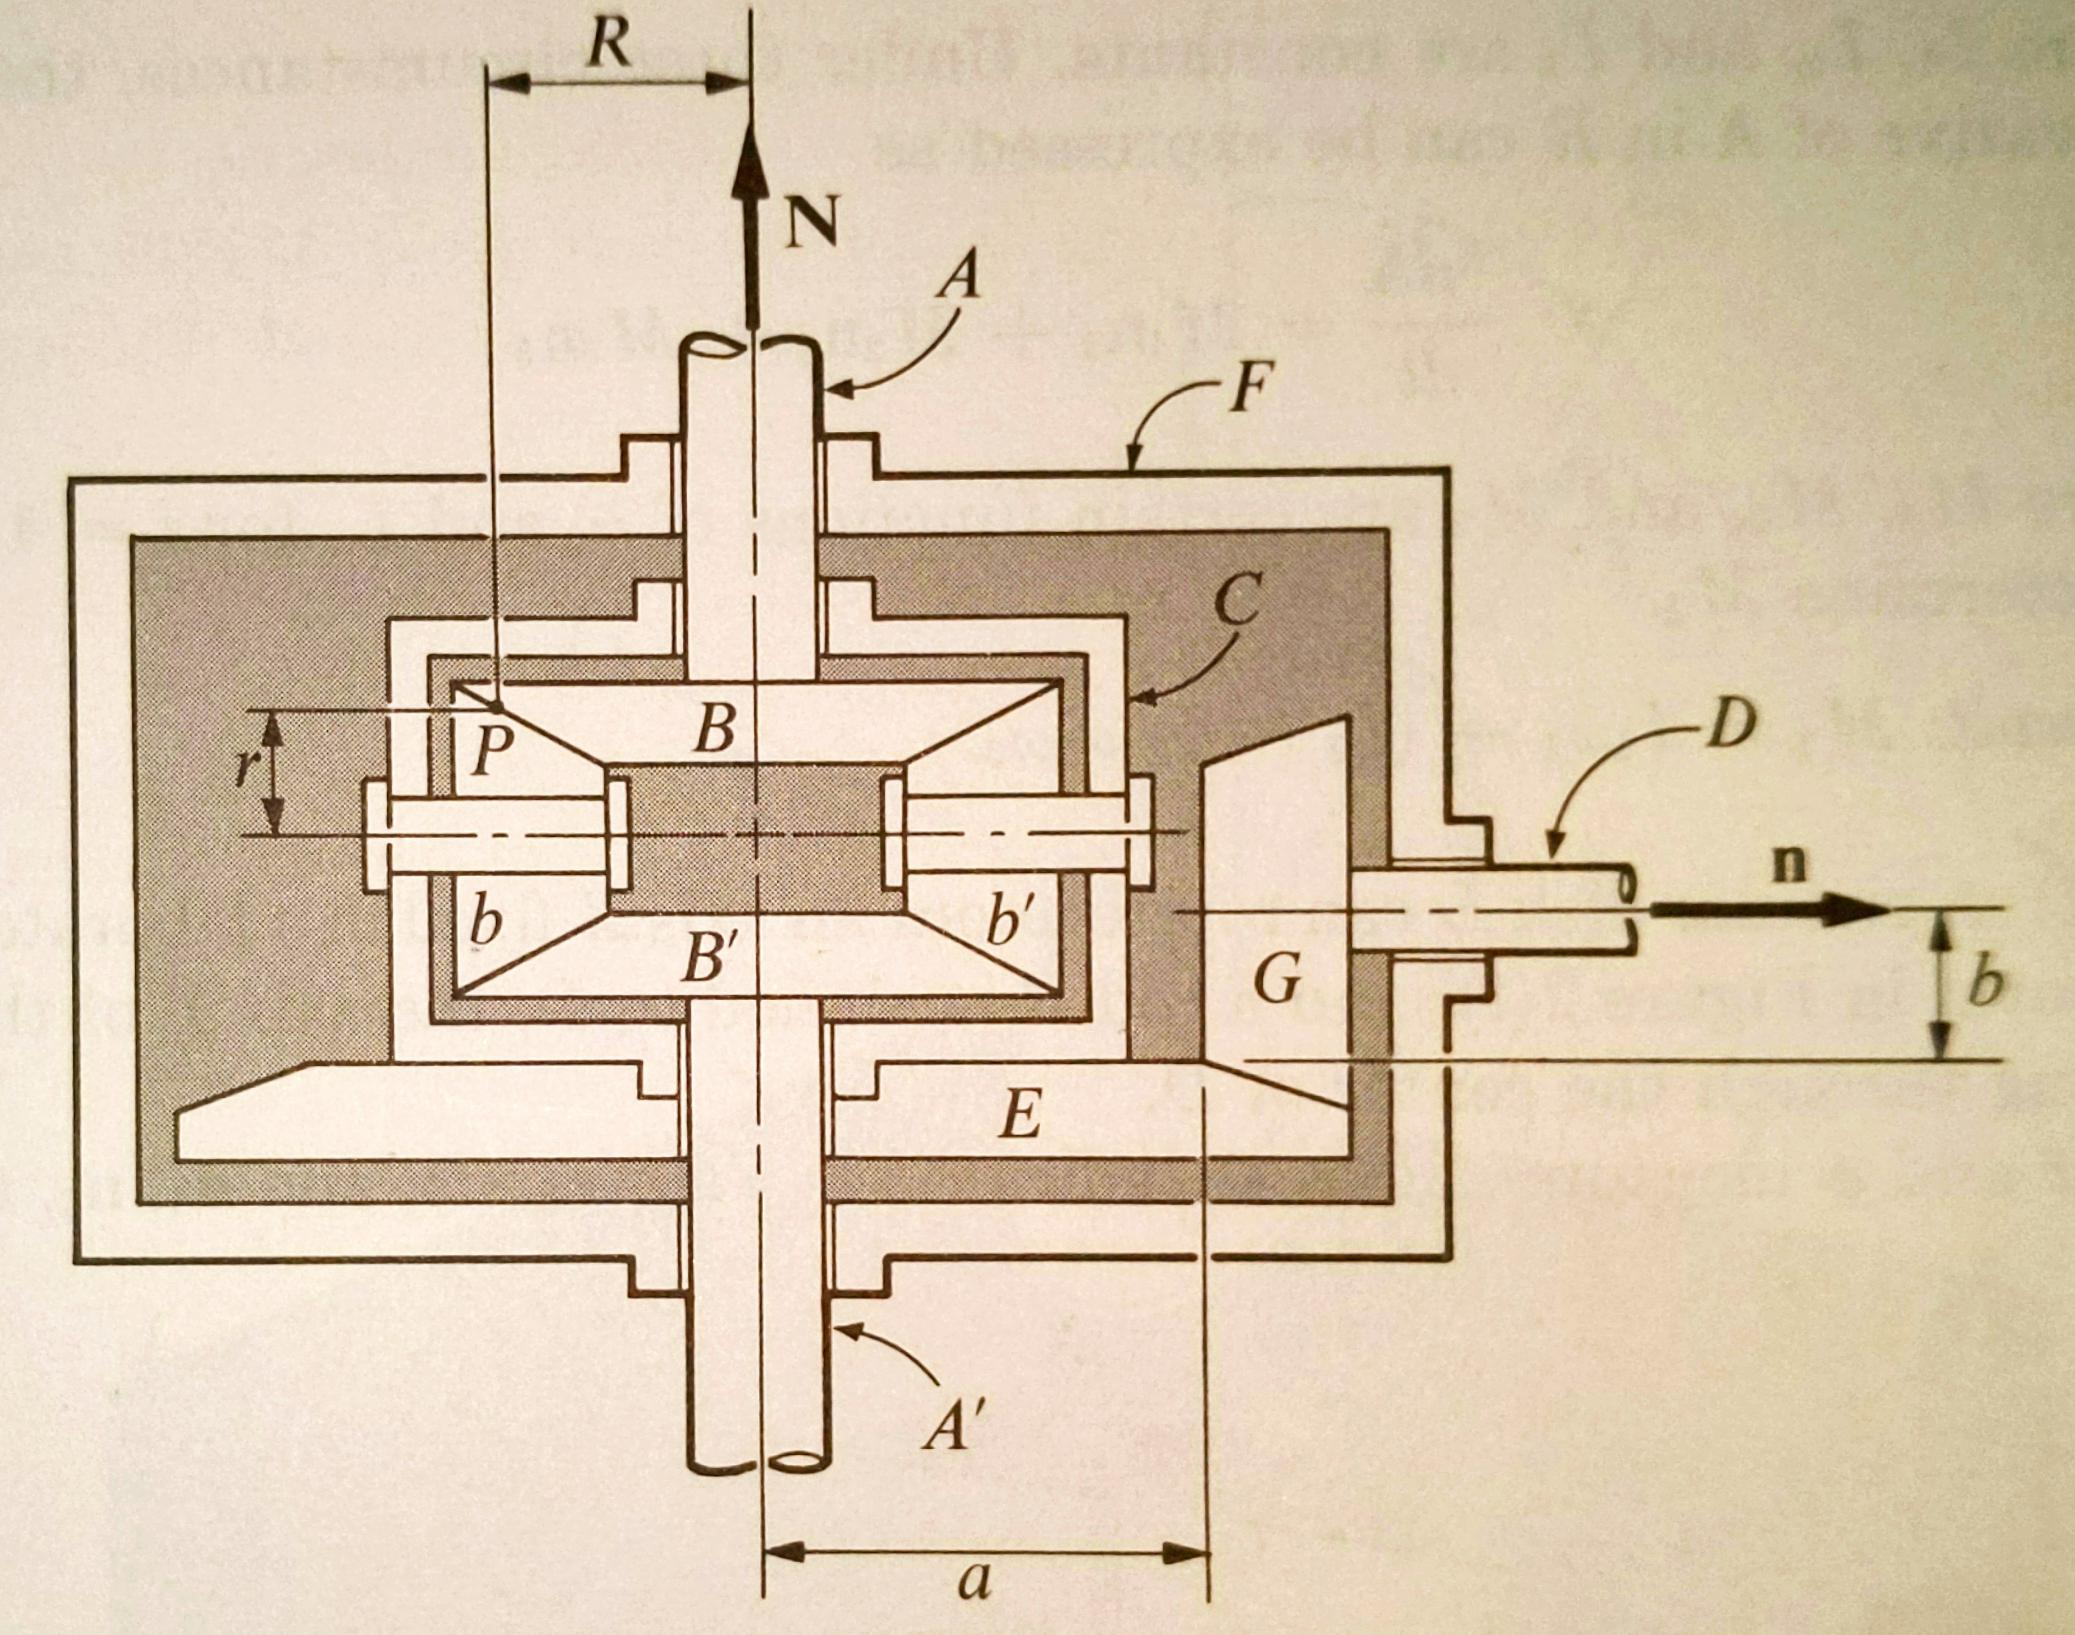
\includegraphics[scale = 0.1]{figs/ProbSet_2/2_d.jpg}
    \caption{}
    \label{2_d}
\end{figure}

\itbf{Mechanism}: Bevel gears $B$ and $B'$ are keyed to $A$ and $A'$, and engage bevel gears $b$ and $b'$, the latter being free to rotate on pins fixed in a casing $C$. $C$ can revolve about the common axis of $A$ and $A'$, and a bevel gear $E$, rigidly attached to $C$, is driven by the gear $G$, which is keyed to the drive shaft $D$.

\bigskip
Given:
\begin{align*}
    \lx{^F}{\pmb \omega}^A &= \Omega \pmb N\\
    \lx{^F}{\pmb \omega}^{A'} &=\Omega' \pmb N\\
    \lx{^F}{\pmb \omega}^D &= \omega \pmb n
\end{align*}

The gears have simple angular velocities w.r.t the frame attached to their shafts. And, the contact points should have same linear velocities. Writing only the magnitudes:
\begin{align*}
    \lx{^F}{\omega}^D b &=  \lx{^F}{\omega}^C a \implies \lx{^F}{\omega}^C  = \frac{b}{a} \omega\\
    \therefore \lx{^F}{\pmb \omega}^C  &= \frac{b}{a} \omega \pmb N\\
\end{align*}

Also,
\begin{align*}
    \lx{^C}{\pmb \omega}^B &= \lx{^F}{\pmb \omega}^B - \lx{^C}{\pmb \omega}^C
    = \lx{^F}{\pmb \omega}^A - \lx{^C}{\pmb \omega}^C = \left( \Omega - \frac{b}{a} \omega \right) \pmb N\\
    %==
     \lx{^C}{\pmb \omega}^{B'} &= \lx{^F}{\pmb \omega}^{B'} - \lx{^C}{\pmb \omega}^C
    = \lx{^F}{\pmb \omega}^{A'} - \lx{^C}{\pmb \omega}^C = \left( \Omega' - \frac{b}{a} \omega \right) \pmb N
\end{align*}

\begin{align*}
    \left . \begin{matrix}
    \lx{^C}{\omega}^{B'} R =  \lx{^C}{\omega}^{b'} r\\
    \lx{^C}{\omega}^{B'} R =  -\lx{^C}{\omega}^{b} r\\
    \lx{^C}{\omega}^{B} R =  -\lx{^C}{\omega}^{b'} r\\
    \lx{^C}{\omega}^{B} R =  \lx{^C}{\omega}^{b} r\\
    \end{matrix} \right \} &\implies \lx{^C}{\omega}^{B'} + \lx{^C}{\omega}^{B} = 0\\
    %===
    &\implies \left( \Omega - \frac{b}{a} \omega \right) + \left( \Omega' - \frac{b}{a} \omega \right) =0 \\
    %==
\end{align*}
$$ \therefore \omega = \frac{a}{2b} \left( \Omega + \Omega' \right)$$

\subsection{2(e) Derivative of angular momentum}
We have,
\begin{align*}
    \lx{^R}{\frac{d \pmb A}{d t}} &= \lx{B}{\frac{d \pmb A}{dt}} + \lx{^R}{\pmb \omega}^B \times A\\
    &=\bm{\dot \omega_1 & \dot \omega_2 & \dot \omega_3} \bm{\pmb n_1 \\ \pmb n_2 \\ \pmb n_3} +
    \left| \begin{matrix} \pmb n_1 & \pmb n_2 &\pmb n_3\\
            \omega_1 & \omega_2 & \omega_3\\
            A_1\omega_1 & A_2 \omega_2 & A_3 \omega_3\\
            \end{matrix} \right|\\
    \text{Let, } \quad \lx{^R}{\frac{d \pmb A}{d t}} &= M_1 \pmb n_1 + M_2 \pmb n_2+ M_3 \pmb n_3\\
    \text{We have, } \quad &\\
    M_1 &= \dot \omega_1 + (I_3 - I_2) \omega_2 \omega_3\\
    M_2 &= \dot \omega_2 + (I_1 - I_3) \omega_1 \omega_3\\
    M_3 &= \dot \omega_3 + (I_2 - I_1) \omega_2 \omega_1\\
\end{align*}

\subsection{2(f) Angular acceleration}
\begin{figure}[H]
    \centering
    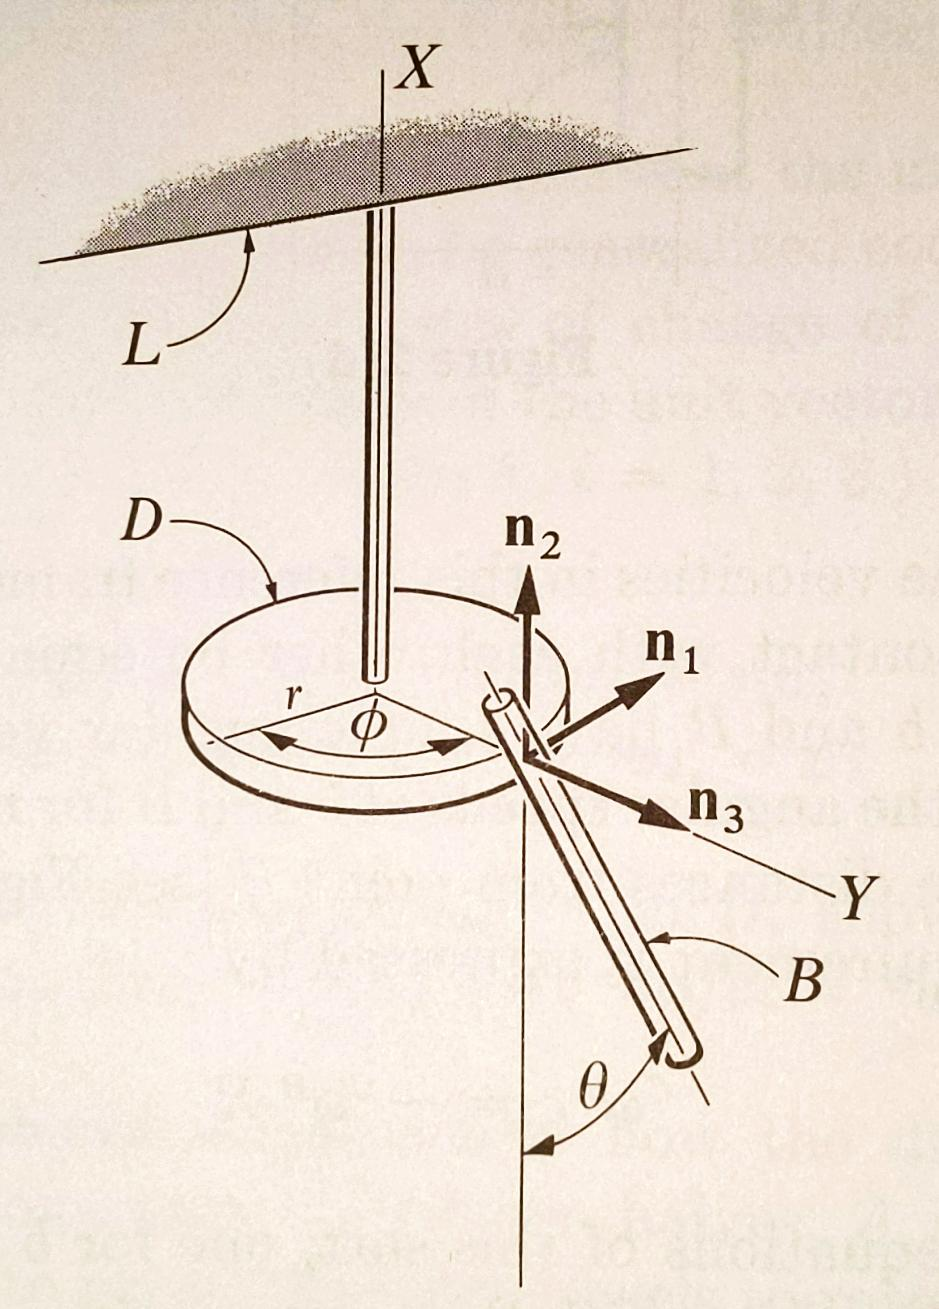
\includegraphics[scale = 0.15]{figs/ProbSet_2/2_f.jpg}
    \caption{}
    \label{2_f}
\end{figure}

\itbf{Sol.}

\begin{align*}
    \lx{^L}{\pmb \omega}{^D} &= \dot \phi \pmb n_2 \qquad and \qquad
    \lx{^L}{\pmb \omega}{^B} = \dot \phi \pmb n_2 + \dot \theta \pmb n_3
\end{align*}

\begin{align*}
    \lx{^L}{\pmb \alpha}{^B} &= \lx{^L}{\frac{d \pmb \omega^B}{d t}}
    %==
    = \lx{^L}{\frac{d}{d t}} \left( \dot \phi \pmb n_2 + \dot \theta \pmb n_3 \right)\\
    %==
    &= \ddot \phi \pmb n_2 + \dot \phi \underbrace{\left( \lx{^L}{\pmb \omega}{^D} \times \pmb n_2 \right)}_{=0} +
    \ddot \theta \pmb n_3 + \dot \theta \underbrace{\left( \lx{^L}{\pmb \omega}{^D} \times \pmb n_3 \right)}_{=\dot \phi n_1}
    %==
    \quad \left[\because \pmb n_1, \pmb n_2, \pmb n_3 \text{ are attached to D (not B)}. \right]\\
    %==
    \implies \lx{^L}{\pmb \alpha}{^B} &= \dot \phi \dot \theta \pmb n_1 + \ddot \phi \pmb n_2 + \ddot \theta \pmb n_2\\
    %===
    \implies& \alpha_1 = \dot \phi \dot \theta, \quad
    \alpha_2 = \ddot \phi, \quad
    \alpha_3 = \ddot \theta
\end{align*}

\subsection{2(g) Angular acceleration of a rolling disk: Choice of  coordinates}
\begin{figure}[H]
    \centering
    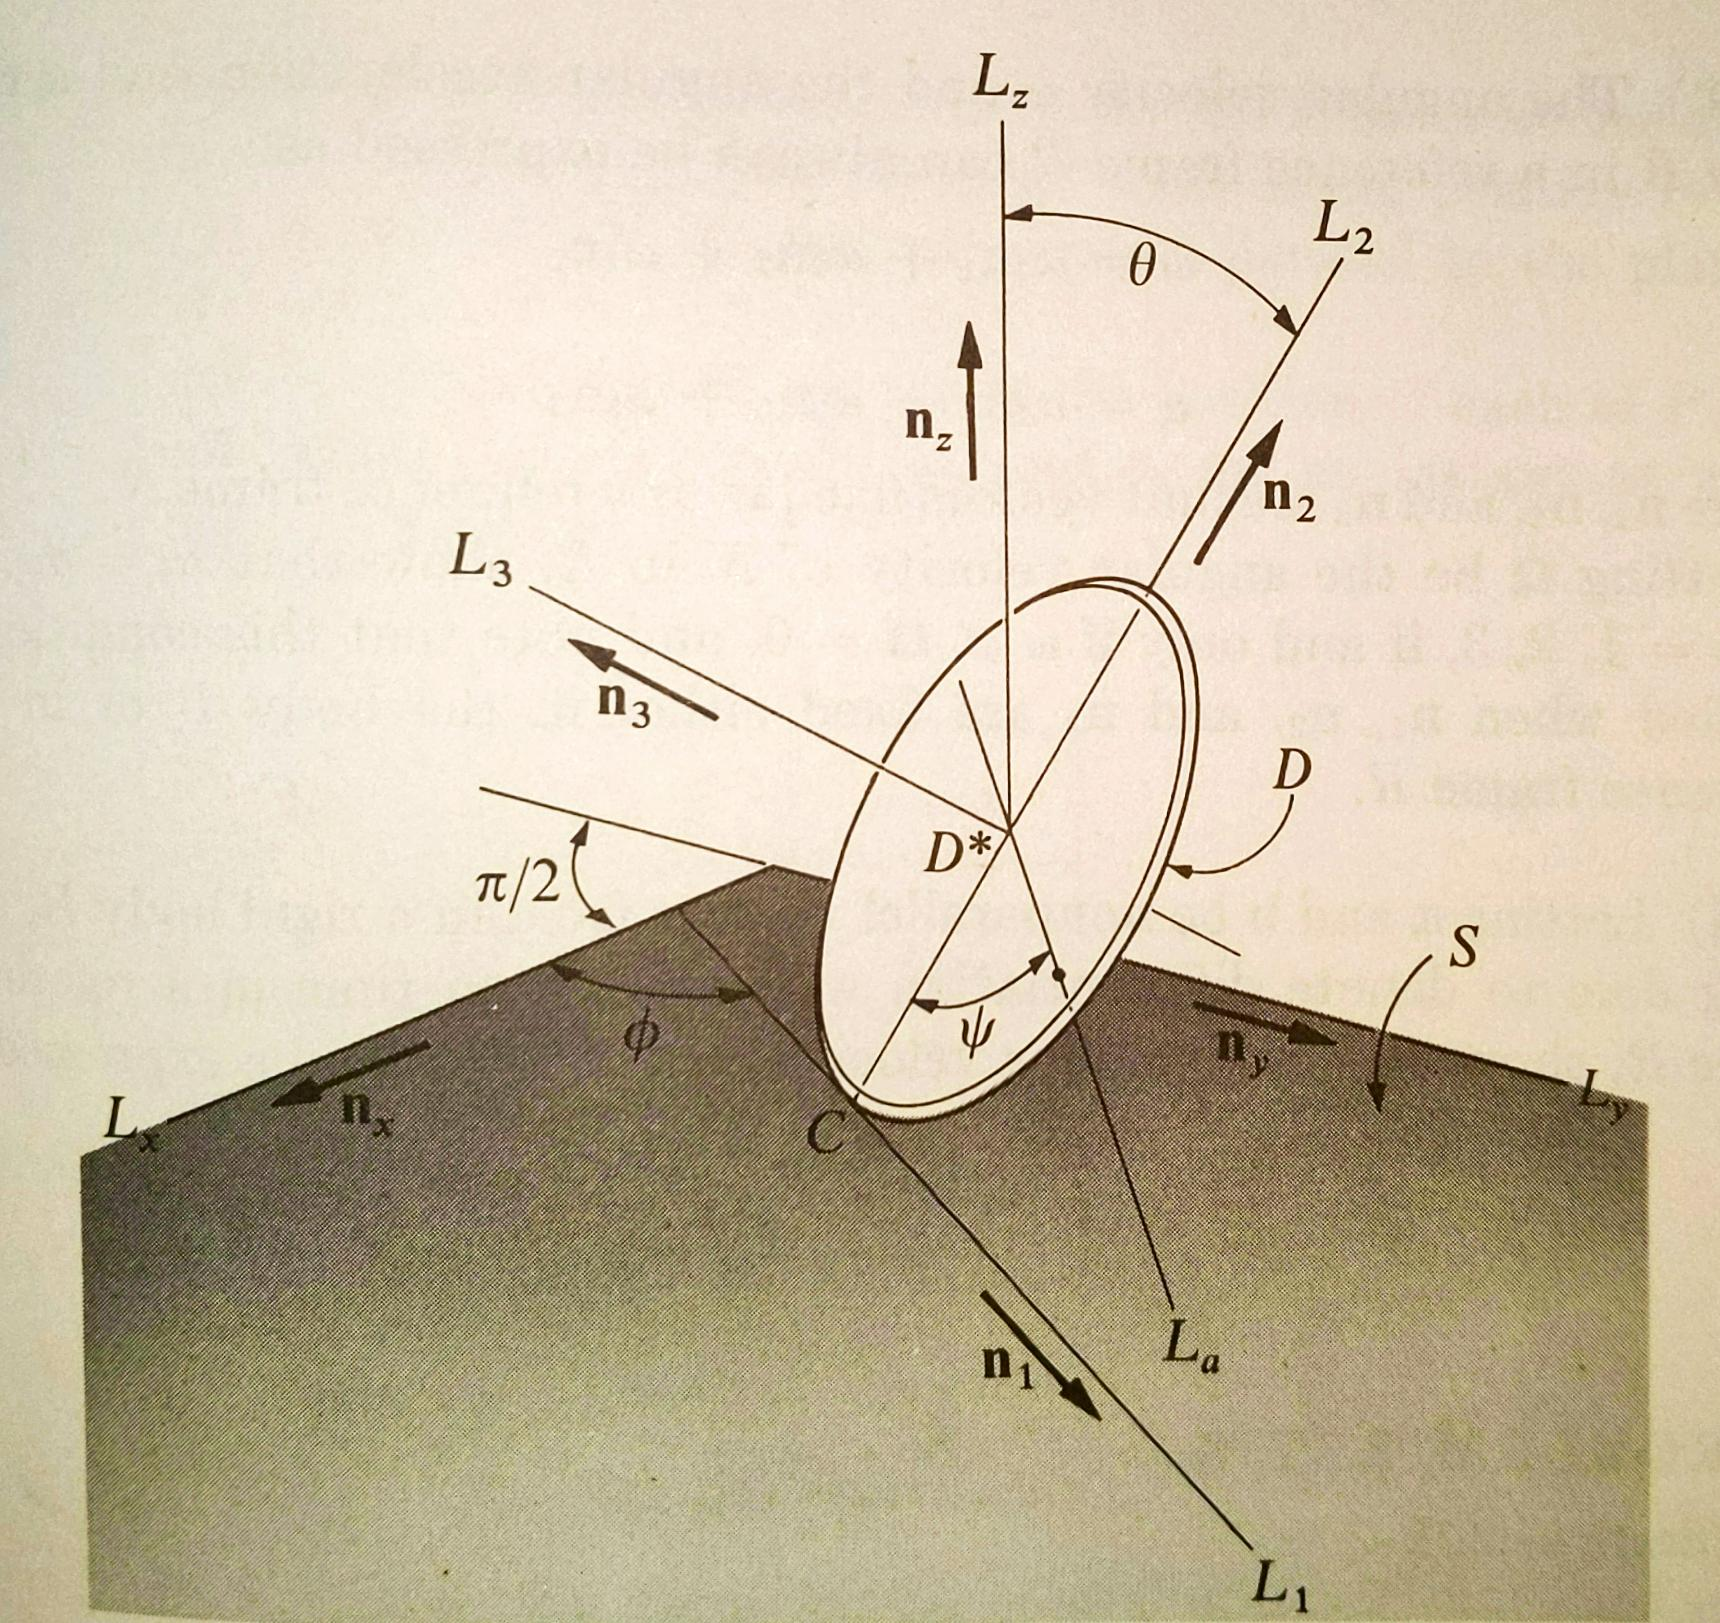
\includegraphics[width=0.7\textwidth, height=0.5\textwidth]{./figs/ProbSet_2/2_g.jpg}
    \caption{}
    \label{2_g}
\end{figure}
The transformation between the two coordinates $\pmb n_1, \pmb n_2, \pmb n_3$ and $\pmb n_x, \pmb n_y, \pmb n_z$ can be written as:
\begin{align*}
    \bm{\pmb n_1 \\ \pmb n_2 \\ \pmb n_3} &= \underbrace{R_1(90 - \theta) R_3(\phi)}_{R} \bm{\pmb n_x \\ \pmb n_y \\ \pmb n_z}\\
    R_1(90 - \theta) &= \bm{1 & 0 & 0 \\
                            0 & \cos (90-\theta) & \sin (90 - \theta) \\
                            0 &-\sin (90 - \theta) & \cos (90 - \theta)}
                      = \bm{1 & 0 & 0\\
                            0 & \sin \theta & \cos \theta \\
                            0 & -\cos \theta & \sin \theta} \\
    R_3(\phi) &= \bm{\cos \phi & \sin \phi & 0\\
                    -\sin \phi & \cos \phi & 0\\
                    0 & 0 & 1}\\
    R &=\bm{1 & 0 & 0\\
            0 & \sin \theta & \cos \theta \\
            0 & -\cos \theta & \sin \theta}
        \bm{\cos \phi & \sin \phi & 0\\
           -\sin \phi & \cos \phi & 0\\
            0 & 0 & 1}
    %==
        = \bm{\cos \phi & \sin \phi & 0\\
              -\sin \theta \sin \phi & \sin \theta \cos \phi & \cos \theta\\
              \cos \theta \sin \phi & -\cos \theta \cos \phi & \sin \theta}\\
    R^{-1} &=(R_1(90 - \theta) R_3(\phi))^{-1} = R_3^{-1} (\phi) R_1^{-1}(90 - \theta) = R_3^{T} (\phi) R_1^{T}(90 - \theta)\\
    &= \bm{\cos \phi & -\sin \phi & 0\\
          \sin \phi & \cos \phi & 0\\
           0 & 0 & 1}
        \bm{1 & 0 & 0\\
           0 & \sin \theta & -\cos \theta \\
           0 & \cos \theta & \sin \theta}
           %==
    = \bm{\cos \phi & - \sin \phi \sin \theta & \sin \phi \cos \theta \\
          \sin \phi & \cos \theta \cos \phi & - \cos \phi \cos \theta \\
          0         & \cos \theta           & \sin \theta }
\end{align*}

\begin{align*}
    \lx{^R}{\pmb \omega}^D &= - \dot \theta \pmb n_1 + \dot \phi \pmb n_z + \dot \psi \pmb n_3
    %===
    = - \dot \theta \pmb n_1 + \dot \phi \cos \theta \pmb n_2 + (\dot \phi \sin \theta + \dot \psi) \pmb n_3
\end{align*}

We have,
\begin{align*}
    \lx{^R}{\pmb \alpha}^B &= \lx{^R}{\frac{d\pmb \omega^B}{dt}}
    %==
    =\lx{^R}{\frac{d}{dt}}\left( - \dot \theta \pmb n_1 + \dot \phi \pmb n_z + \dot \psi \pmb n_3 \right)
    %==
    = - \ddot \theta \pmb n_1 - \dot \theta \dot{\pmb n}_1
       + \ddot \phi \pmb n_z + \dot \phi \dot{\pmb n}_z
       + \ddot \psi \pmb n_3 + \dot \psi \dot{\pmb n}_3
\end{align*}

also,
\begin{align*}
    \lx{^R}{\frac{d \pmb n_1}{dt}} &= \lx{^R}{\pmb \omega}^{L_1} \times \pmb n_1 = \dot \phi \pmb n_z \times \pmb n_1 = \dot \phi (\cos \theta \pmb n_2 + \sin \theta \pmb n_3) \times \pmb n_1\\
    &= \dot \phi (-\cos \theta \pmb n_3 +\sin \theta  \pmb n_2) \\
    %==
    \lx{^R}{\frac{d \pmb n_z}{dt}} &= 0 \qquad [\because \pmb n_z \text{ is fixed to the frame } R]
    \\
    %==
    \lx{^R}{\frac{d \pmb n_3}{dt}} &=  \lx{^R}{\pmb \omega}^{L_3} \times \pmb n_3
    = (\dot \phi \pmb n_z - \dot \theta \pmb n_1 ) \times \pmb n_3
    = (\dot \phi (\cos \theta \pmb n_2 + \sin \theta \pmb n_3) - \dot \theta \pmb n_1 ) \times \pmb n_3\\
    &= \dot \phi \cos \theta \pmb n_1 + \dot \theta \pmb n_2
\end{align*}

Substituting,
\begin{align*}
    \lx{^R}{\pmb \alpha}^B &=
       - \ddot \theta \pmb n_1 - \dot \theta (\dot \phi (-\cos \theta \pmb n_3 +\sin \theta  \pmb n_2) )
       + \ddot \phi (\cos \theta \pmb n_2 + \sin \theta \pmb n_3)
       + \ddot \psi \pmb n_3 + \dot \psi ( \dot \phi \cos \theta \pmb n_1 + \dot \theta \pmb n_2)\\
       &= \bm{
            \underbrace{
            -\ddot \theta + \dot \phi \dot \theta \cos \theta}_{\alpha_1} &
            \underbrace{
            -\dot \theta \dot \phi \sin \theta + \ddot \phi \cos \theta + \dot \psi \dot \theta }_{\alpha_2} &
            \underbrace{
            \dot \theta \dot \phi \cos \theta + \ddot \phi \sin \theta + \ddot \psi}_{\alpha_3}}
       \bm{\pmb n_1 \\ \pmb n_2 \\ \pmb n_3}\\
       %====
       &= \bm{\alpha_1 & \alpha_2 & \alpha_3} R
       \bm{\pmb n_x \\ \pmb n_y \\ \pmb n_z}
       %==
        = \bm{\alpha_1 & \alpha_2 & \alpha_3}
          \bm{\cos \phi & \sin \phi & 0\\
              -\sin \theta \sin \phi & \sin \theta \cos \phi & \cos \theta\\
              \cos \theta \sin \phi & -\cos \theta \cos \phi & \sin \theta}
            \bm{\pmb n_x \\ \pmb n_y \\ \pmb n_z}\\
        %==
        &= \bm{
            \alpha _1 \cos \phi - \alpha_2 \sin \theta \sin \phi + \alpha_3 \cos \theta \cos \phi &(=\alpha_x) \\
            \alpha_1 \sin \phi + \alpha_2 \sin \theta \cos \phi - \alpha_3 \cos \theta \cos \phi & (= \alpha_y)\\
            \alpha_2 \cos \theta + \alpha_3 \sin \theta & (=\alpha_z)}^T
        \bm{\pmb n_x \\ \pmb n_y \\ \pmb n_z}
\end{align*}

alternately,
\begin{align*}
    \lx{^R}{\pmb \omega}^D &= - \dot \theta \pmb n_1 + \dot \phi \pmb n_z + \dot \psi \pmb n_3\\
    %===
    &=-\dot \theta (\cos \phi \pmb n_x + \sin \phi \pmb n_y) + \dot \phi \pmb n_z + \dot \psi (\cos \theta \sin \phi \pmb n_x  -\cos \theta \cos \phi \pmb n_y  + \sin \theta \pmb n_z)\\
    %===
    &=\bm{-\dot \theta \cos \phi + \dot \psi \cos \theta \sin \phi &
         -\dot \theta \sin \phi - \dot \psi \cos \theta \cos \phi &
         \dot \phi + \dot \psi \sin \theta }
        \bm{\pmb n_x \\ \pmb n_y \\ \pmb n_z}
\end{align*}

Thus,
\begin{align*}
     \lx{^R}{\pmb \alpha}^B &= \lx{^R}{\frac{d\pmb \omega^B}{dt}}
     = \lx{^R}{\frac{d}{dt}} \left(\bm{-\dot \theta \cos \phi + \dot \psi \cos \theta \sin \phi &
         -\dot \theta \sin \phi - \dot \psi \cos \theta \cos \phi &
         \dot \phi + \dot \psi \sin \theta }
    \right) \bm{\pmb n_x \\ \pmb n_y \\ \pmb n_z}\\
    %==
    &=\bm{
        -\ddot \theta \cos \phi + \ddot \psi \cos \theta sin \phi + \dot \theta \dot \phi \sin \phi + \dot \psi \dot \phi \cos \theta \cos \phi - \dot \psi \dot \theta \cos \theta \sin \phi & (= \alpha_x)\\
        %==
        -\ddot \theta \sin \phi - \ddot \psi \cos \theta \cos \phi - \dot \theta \dot \phi \cos \phi + \dot \psi \dot \theta \sin \theta \cos \phi + \dot \psi \dot \phi \cos \theta \sin \phi & (= \alpha_y)\\
        %==
        \ddot \phi + \ddot \psi \sin \theta + \dot \psi \dot \theta \cos \theta & (=\alpha_z)
    }^T
    \bm{\pmb n_x \\ \pmb n_y \\ \pmb n_z}\\
\end{align*}

\itbf{Note:}
\begin{itemize}
    \item We can not just take $d \pmb n_z/dt$ as $\omega \times \pmb n_z$ in $\pmb n_1, \pmb n_2, \pmb n_3$ coordinates as $\pmb n_z$ is not rigidly fixed to the coordinates. This is only possible when $\pmb n_z$ does't change with time in $\pmb n_1, \pmb n_2, \pmb n_3$ frame. But once, the differentiation is done, one vector in $\pmb n_1, \pmb n_2, \pmb n_3$ frame can be written in $\pmb n_x, \pmb n_y, \pmb n_z$ frame using transformation matrices as they are instantaneous.

    \item Thus the rotation transformation can be used after differentiation as well.
\end{itemize}

\subsection{2(h) $\alpha$ when body and frame have paraller $\omega$'s}
Given, $\{\pmb n_1, \pmb n_2, \pmb n_3 \} \in N$ has an angular velocity $\Omega$ in R, and
\begin{align*}
    \lx{^R}{\pmb \omega}^B &= \omega_1 \pmb n_1 + \omega_2 \pmb n_2 + \omega_3 \pmb n_3\\
    \lx{^R}{\pmb \alpha}^B &= \alpha_1 \pmb n_1 + \alpha_2 \pmb n_2 + \alpha_3 \pmb n_3\\
    \text{and,}\qquad \alpha_i &= d \omega_i/dt = \dot \omega_i
\end{align*}
Consider,
\begin{align*}
    \lx{^R}{\pmb \alpha}^B &= \lx{^R}{\frac{d\pmb \omega^B}{dt}} =\sum_{i=1}^3 \left( \dot \omega_i\pmb n_i + \omega_i \lx{^R}{\frac{d\pmb n_i}{dt}} \right)
    = \sum_{i=1}^3 \left( \alpha_i \pmb n_i + \omega_i \lx{^R}{\frac{d\pmb n_i}{dt}} \right) = \lx{^R}{\pmb \alpha}^B + \sum_{i=1}^3 \left(\omega_i \lx{^R}{\frac{d\pmb n_i}{dt}} \right)\\
    &\qquad \qquad  \iff \sum_{i=1}^3 \left(\omega_i \lx{^R}{\frac{d\pmb n_i}{dt}} \right) = 0
\end{align*}
We have,
\begin{align*}
    \sum_{i=1}^3 \left(\omega_i \lx{^R}{\frac{d\pmb n_i}{dt}} \right) &
    = \sum_{i=1}^3 \left(\omega_i (\Omega \times \pmb n_i) \right)
    = \Omega \times ( \omega_1 \pmb n_1 + \omega_2 \pmb n_2 + \omega_3 \pmb n_3)
    = \Omega \times \pmb \omega
\end{align*}
thus,
\begin{align*}
    \alpha_i &=\frac{d \omega_i}{dt}, \; for \; i = 1,2,3 \; \iff \Omega \times \pmb \omega = 0 &q.e.d
\end{align*}

\subsection{2(i) $\pmb \omega = (\dot{\pmb a} \times \dot{\pmb b}) / (\dot{\pmb a} . \pmb b)$}

Consider,
\begin{align*}
    \dot{\pmb a} \times \dot{\pmb b} &= \dot{\pmb a} \times (\pmb \omega \times \pmb b) = (\dot{\pmb a}.\pmb b)\pmb \omega - \underbrace{(\dot{\pmb a} . \pmb \omega)}_{=0} \pmb b
    %===
    \qquad
    \bm{\because& \pmb a \times (\pmb b \times \pmb c) = (\pmb a.\pmb c)\pmb b - (\pmb a.\pmb b)\pmb c\\
    \because& (\pmb \omega \times \pmb a) \times \pmb \omega = 0 }\\
    %===
    \implies \pmb \omega &= \frac{\dot{\pmb a} \times \dot{\pmb b}}{(\dot{\pmb a}.\pmb b)} &q.e.d
\end{align*}

%===============================================================================
\newpage
\section{Problem Set 3}
KJDSAFF

\input{ProblemSets/ProbSet_3/3b.tex}
\input{ProblemSets/ProbSet_3/3c.tex}
\input{ProblemSets/ProbSet_3/3d.tex}
\input{ProblemSets/ProbSet_3/3e.tex}
\input{ProblemSets/ProbSet_3/3f.tex}
\input{ProblemSets/ProbSet_3/3g.tex}
\input{ProblemSets/ProbSet_3/3h.tex}
\input{ProblemSets/ProbSet_3/3i.tex}
\input{ProblemSets/ProbSet_3/3j.tex}
\input{ProblemSets/ProbSet_3/3k.tex}
\input{ProblemSets/ProbSet_3/3l.tex}
%===============================================================================
\newpage


\end{document}
